%%%%%%%%%%%%%%%%%%%%%%%%%%%%%%%%%%%%%%%%%
% Short Sectioned Assignment LaTeX Template Version 1.0 (5/5/12)
% This template has been downloaded from: http://www.LaTeXTemplates.com
% Original author:  Frits Wenneker (http://www.howtotex.com)
% License: CC BY-NC-SA 3.0 (http://creativecommons.org/licenses/by-nc-sa/3.0/)
%%%%%%%%%%%%%%%%%%%%%%%%%%%%%%%%%%%%%%%%%

%----------------------------------------------------------------------------------------
%	PACKAGES AND OTHER DOCUMENT CONFIGURATIONS
%----------------------------------------------------------------------------------------

\documentclass[paper=a4, fontsize=11pt]{scrartcl} % A4 paper and 11pt font size

% ---- Entrada y salida de texto -----

\usepackage[T1]{fontenc} % Use 8-bit encoding that has 256 glyphs
\usepackage[utf8]{inputenc}
%\usepackage{fourier} % Use the Adobe Utopia font for the document - comment this line to return to the LaTeX default

% ---- Idioma --------

\usepackage[spanish, es-tabla]{babel} % Selecciona el español para palabras introducidas automáticamente, p.ej. "septiembre" en la fecha y especifica que se use la palabra Tabla en vez de Cuadro

% ---- Otros paquetes ----

\usepackage{amsmath,amsfonts,amsthm} % Math packages
%\usepackage{graphics,graphicx, floatrow} %para incluir imágenes y notas en las imágenes
\usepackage{graphics,graphicx, float} %para incluir imágenes y colocarlas

% Para hacer tablas comlejas
%\usepackage{multirow}
%\usepackage{threeparttable}

%\usepackage{sectsty} % Allows customizing section commands
%\allsectionsfont{\centering \normalfont\scshape} % Make all sections centered, the default font and small caps

\usepackage{fancyhdr} % Custom headers and footers
\pagestyle{fancyplain} % Makes all pages in the document conform to the custom headers and footers
\fancyhead{} % No page header - if you want one, create it in the same way as the footers below
\fancyfoot[L]{} % Empty left footer
\fancyfoot[C]{} % Empty center footer
\fancyfoot[R]{\thepage} % Page numbering for right footer
\renewcommand{\headrulewidth}{0pt} % Remove header underlines
\renewcommand{\footrulewidth}{0pt} % Remove footer underlines
\setlength{\headheight}{13.6pt} % Customize the height of the header

\numberwithin{equation}{section} % Number equations within sections (i.e. 1.1, 1.2, 2.1, 2.2 instead of 1, 2, 3, 4)
\numberwithin{figure}{section} % Number figures within sections (i.e. 1.1, 1.2, 2.1, 2.2 instead of 1, 2, 3, 4)
\numberwithin{table}{section} % Number tables within sections (i.e. 1.1, 1.2, 2.1, 2.2 instead of 1, 2, 3, 4)

\setlength\parindent{0pt} % Removes all indentation from paragraphs - comment this line for an assignment with lots of text

\newcommand{\horrule}[1]{\rule{\linewidth}{#1}} % Create horizontal rule command with 1 argument of height


%----------------------------------------------------------------------------------------
%	TÍTULO Y DATOS DEL ALUMNO
%----------------------------------------------------------------------------------------

\title{	
\normalfont \normalsize 
\textsc{{\bf Ingeniería de Servidores (2014-2015)} \\ Grado en Ingeniería Informática \\ Universidad de Granada} \\ [25pt] % Your university, school and/or department name(s)
\horrule{0.5pt} \\[0.4cm] % Thin top horizontal rule
\huge Memoria Práctica 5 \\ % The assignment title
\horrule{2pt} \\[0.5cm] % Thick bottom horizontal rule
}

\author{José Arcos Aneas} % Nombre y apellidos

\date{\normalsize\today} % Incluye la fecha actual

%----------------------------------------------------------------------------------------
% DOCUMENTO
%----------------------------------------------------------------------------------------

\begin{document}

\maketitle % Muestra el Título

\newpage %inserta un salto de página

\tableofcontents % para generar el índice de contenidos

\newpage

%----------------------------------------------------------------------------------------
%	Cuesti´on 1
%----------------------------------------------------------------------------------------

\section{Al modificar los valores del kernel de este modo, no logramos que persistan después de reiniciar la máquina. ¿Qué archivo hay que editar para que los cambios sean permanentes?}

El fichero que hay que modificar es el “/etc/sysctln.conf”.

\section{ ¿Con qué opción se muestran todos los parámetros modificables en tiempo de ejecución? Elija dos parámetros y expliqué, en dos líneas, qué función tienen.}

La opción “–a” nos permite ver todos los valores de las variables del kernel. 
La opción “–w” nos permite modificar los parámetros de forma temporal. 
Y la opción “–p” nos sirve para que se carguen los valores del fichero "sysctl.conf" si no 
se le ha dado ninguno.


\section{Realice una copia de seguridad del registro y restaurela, ilustre el proceso con capturas.}
\footnote{http://support.microsoft.com/kb/326216/es}
\footnote{http://support.microsoft.com/kb/322756/es-es}

Primero abrimos el asistente que encontramos en todas las versiones de Windows.

\begin{figure}[H]
\begin{center}
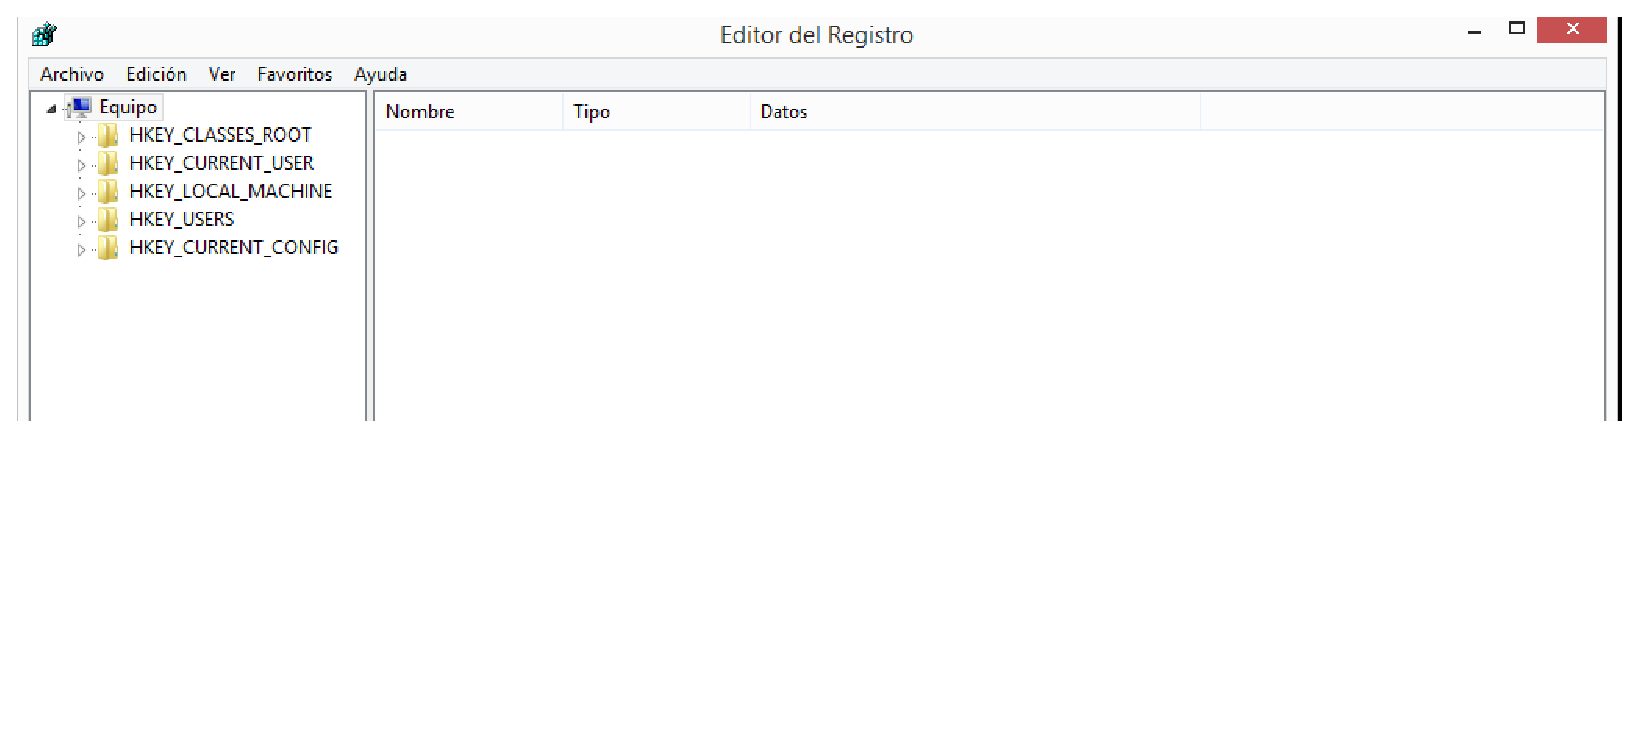
\includegraphics[scale=0.4]{imagenes/cuestion3-1.eps}
\caption{Inicio asistente del registro.}
\end{center}
\end{figure}

En la ventana anterior seleccionamos el registro del que deseamos crear una copia de seguridad.

Pulsamos en inicio y en exportar.
\begin{figure}[H]
\begin{center}
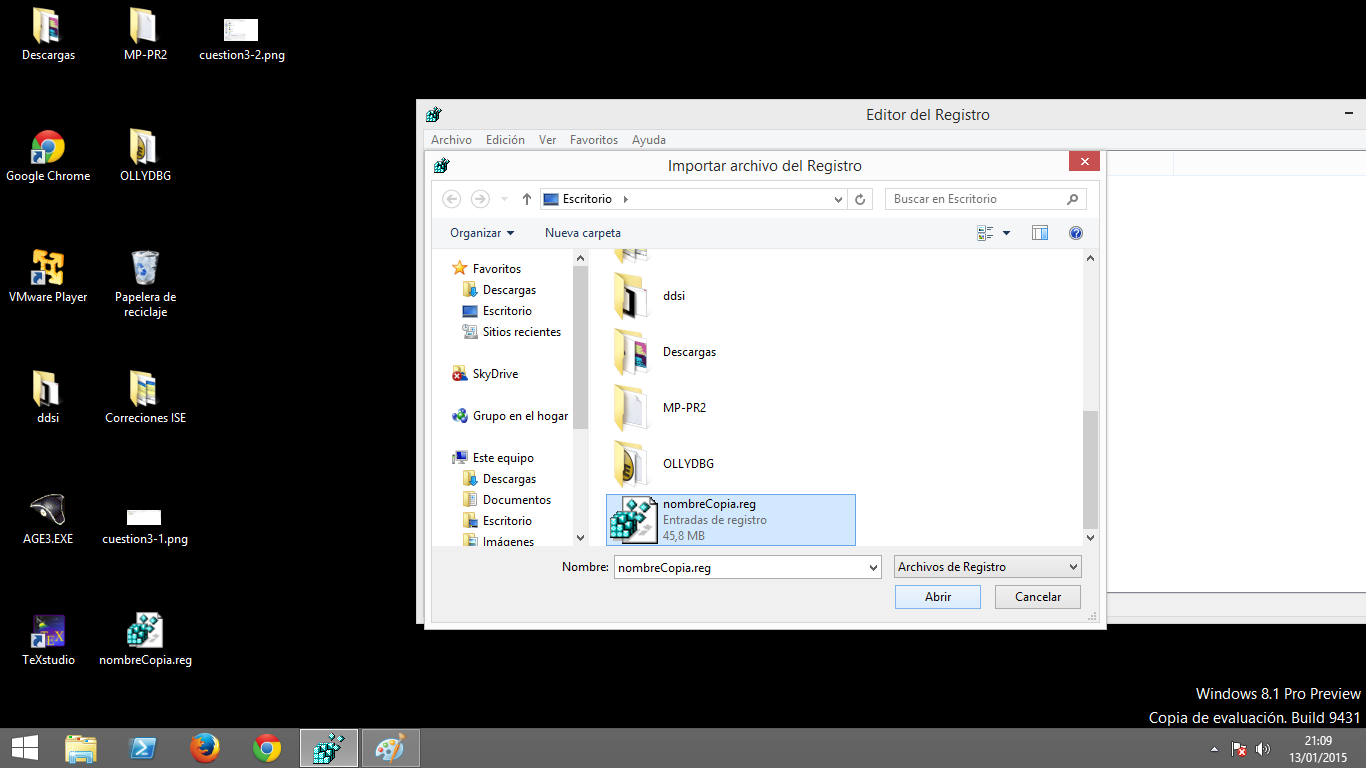
\includegraphics[scale=0.4]{imagenes/cuestion3-2.eps}
\caption{Exportar copia de seguridad del registro.}
\end{center}
\end{figure}

Una vez le demos un nombre podrémos guardarlo y listo.

Ahora para cargarlos debemos abrir de nuevo el asistente y pulsar en inicio, y en importar. En la siguiente ventana seleccionar el elemento que deseamos restaurar y listo.
\begin{figure}[H]
\begin{center}
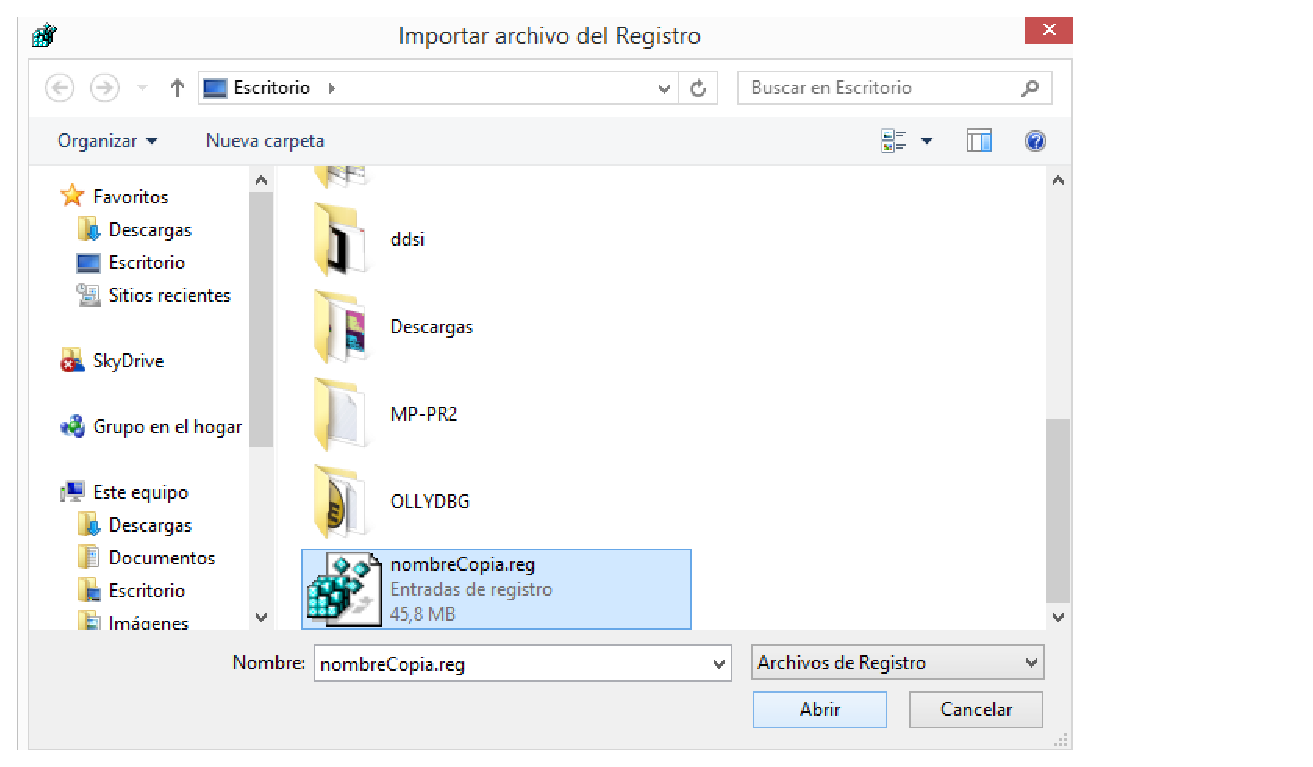
\includegraphics[scale=0.8]{imagenes/cuestion3-3.eps}
\caption{Restauración de copia de registro.}
\end{center}
\end{figure}

\section{¿Cómo se abre una consola en Windows? ¿Qué comando hay que ejecutar para editar el registro? Muestre su ejecución con capturas de pantalla.}
Enlace de interés \footnote{http://norfipc.com/inf/comandos-consola-windows-7.html}
Con el comando CMD, para la consola de Windows. O podemos pulsar la tecla de Windows +R
\begin{figure}[H]
\begin{center}
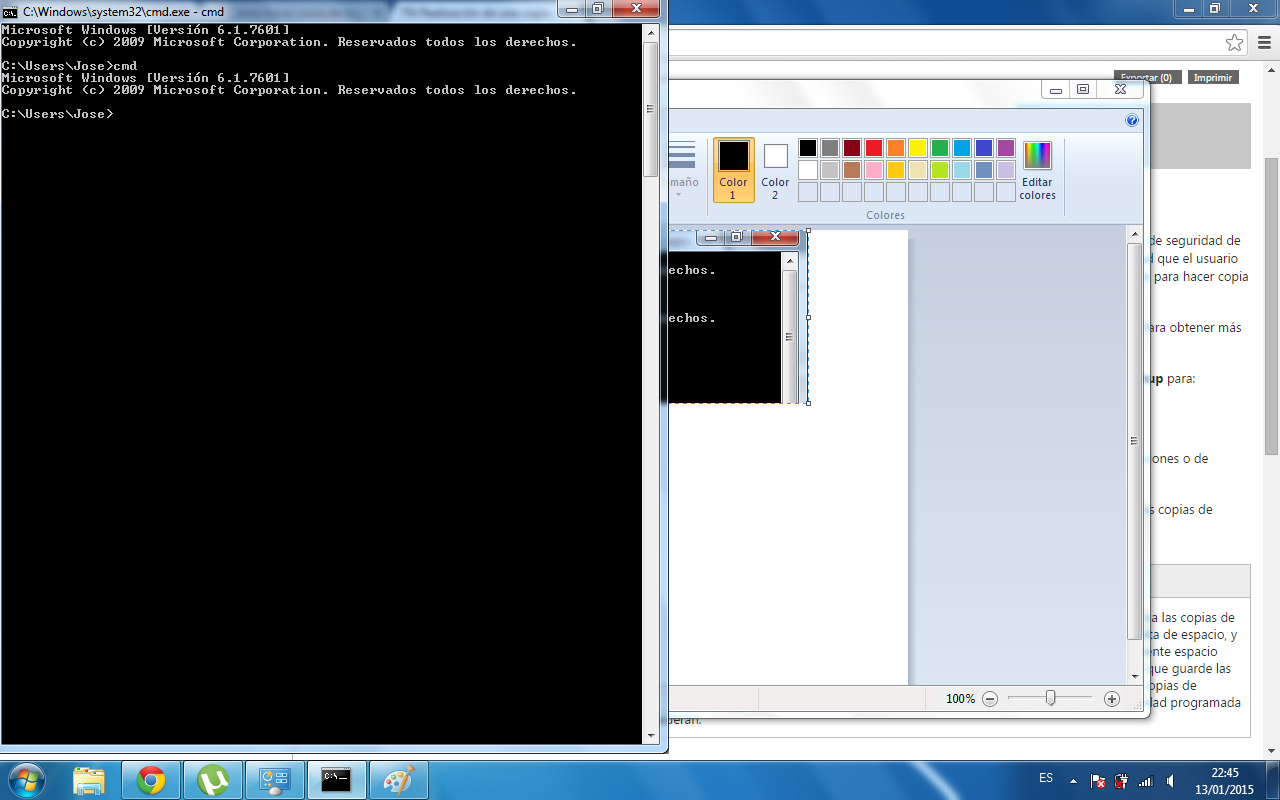
\includegraphics[scale=0.4]{imagenes/cuestion4-1.eps}
\caption{Inicio consola de windows.}
\end{center}
\end{figure}


El comando siguiente para poder ejecutar la interfaz del registro sería “regedit”.
\begin{figure}[H]
\begin{center}
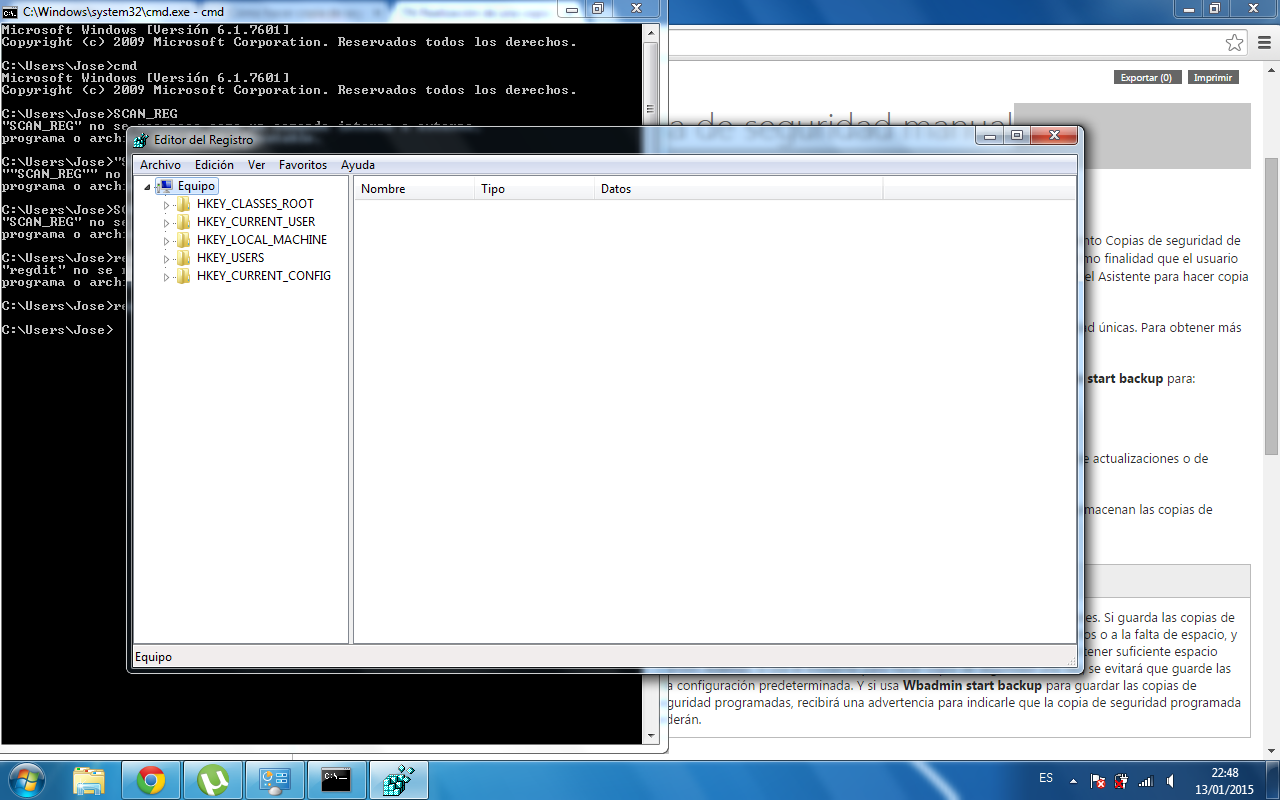
\includegraphics[scale=0.3]{imagenes/cuestion4-2.eps}
\caption{Inicio asistente de registro.}
\end{center}
\end{figure} 

\subsection{¿Qué tecla hay que pulsar para poder restaurar el registro?} 
Para restaurar un registro anterior podemos pulsar inicio y exportar.

\section{Las cadenas de caracteres y valores numéricos tienen distintos tipos. Busque en la documentación de Microsoft y liste todos los tipos de valores.}

La siguiente tabla la realice el año pasado, y la he copiado.

\begin{figure}[H]
\begin{center}
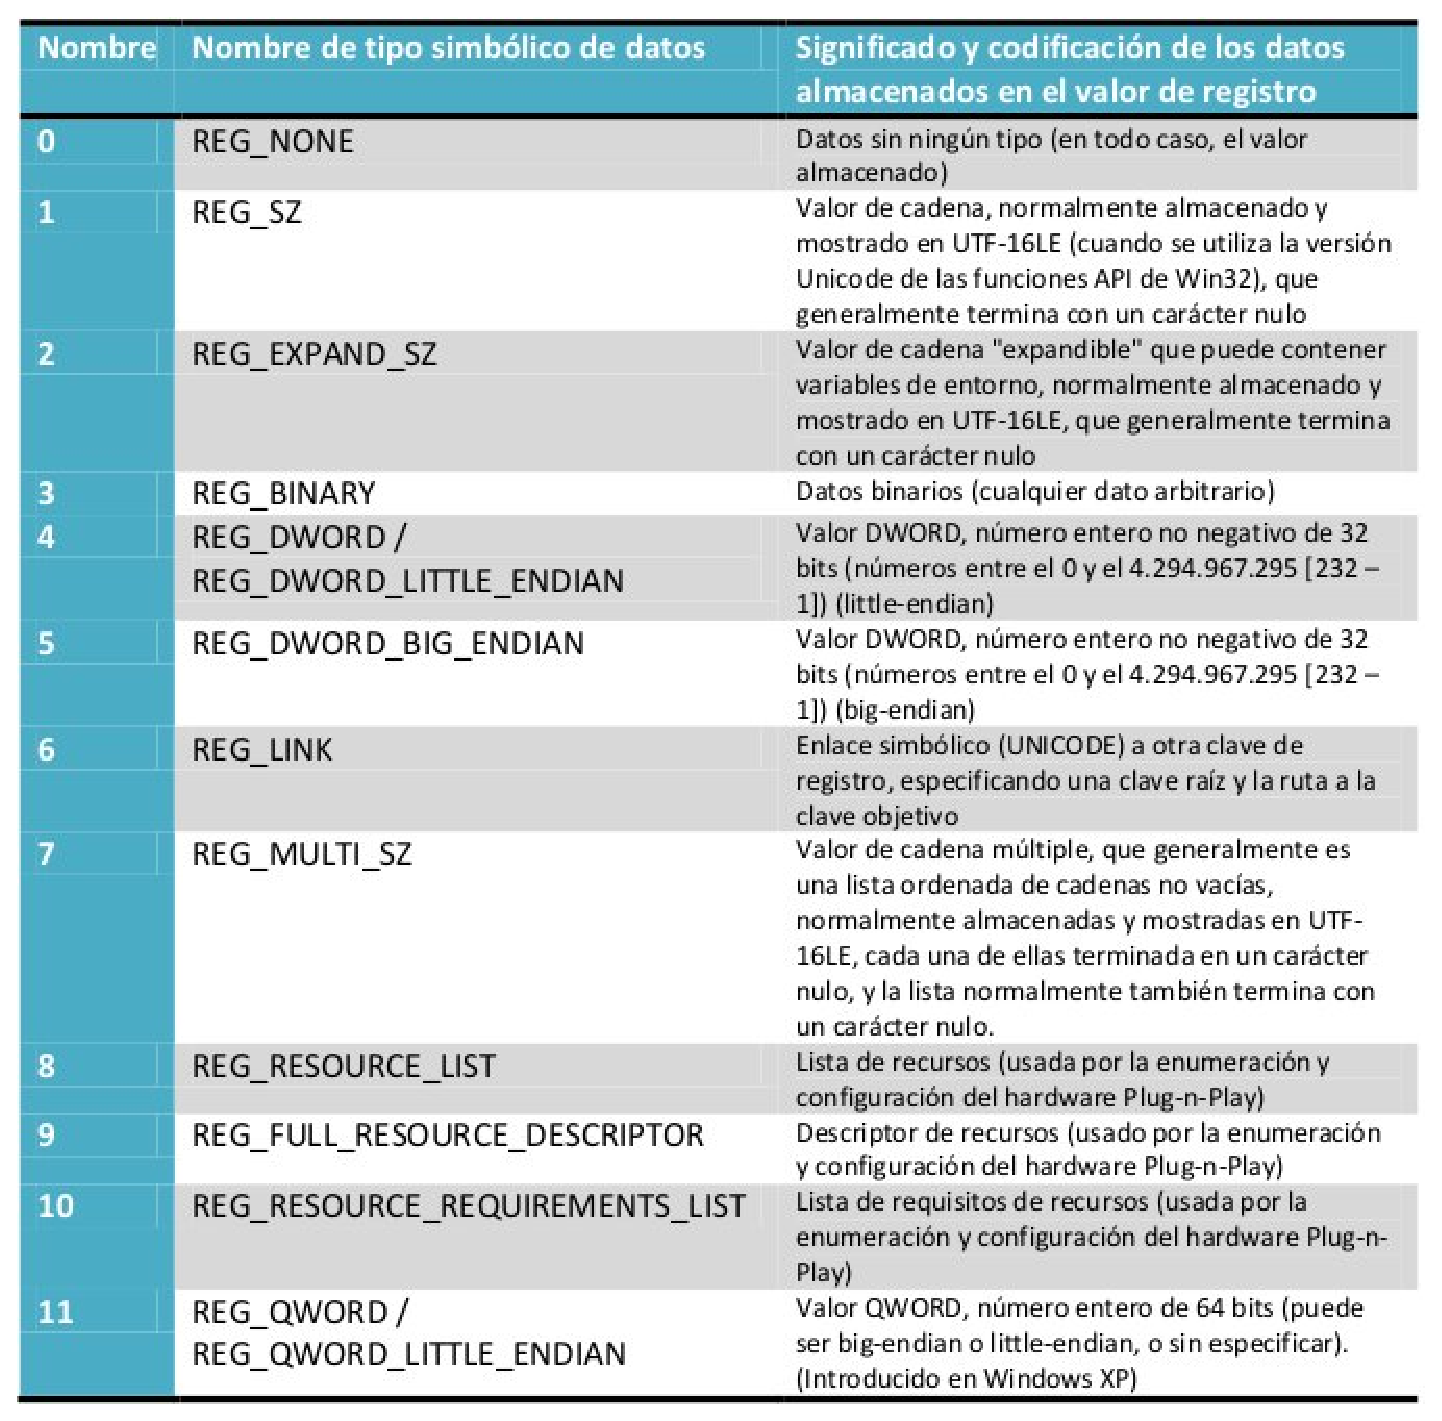
\includegraphics[scale=0.4]{imagenes/cuestion5.eps}
\caption{Lista de los tipos de valores.}
\end{center}
\end{figure}


\section{Enumere qué elementos se pueden configurar en Apache y en IIS para que Moodle funcione mejor.}
\footnote{http://httpd.apache.org/docs/2.0/es/sections.html}
\footnote{http://support.microsoft.com/kb/323972/es}
Apache: Se pueden modificar el máximo de clientes, el número de módulos que 
Apache carga (en el fichero httpd.conf), máximo de peticiones por cliente, utilizar 
indices de directoros correctamente, para evitar "negociación de contenidos", un 
timeout de 30 a 60 segundos, entre otros. 
IIS: Se puede mejorar el "ListenBackLog" entre 2 y 5. El tamaño de la memoria que se 
va a usar, el tamaño máximo de los ficheros de cache, se puede crear un 
ObjectCacheTTL para cambiar el intervalo de tiempo que los ficheros en caché se van a 
mantener ahí.

\section{Ajuste la compresión en el servidor y analice su comportamiento usando varios valores para el tamaño a de archivo partir del cual comprimir. Para comprobar que está comprimiendo puede usar el navegador o comandos como curl (see url) o lynx. Muestre capturas de pantalla de todo el proceso.}

Lo primero que vamos a ver es que, las cabeceras aparecén con ningun valor.

\begin{figure}[H]
\begin{center}
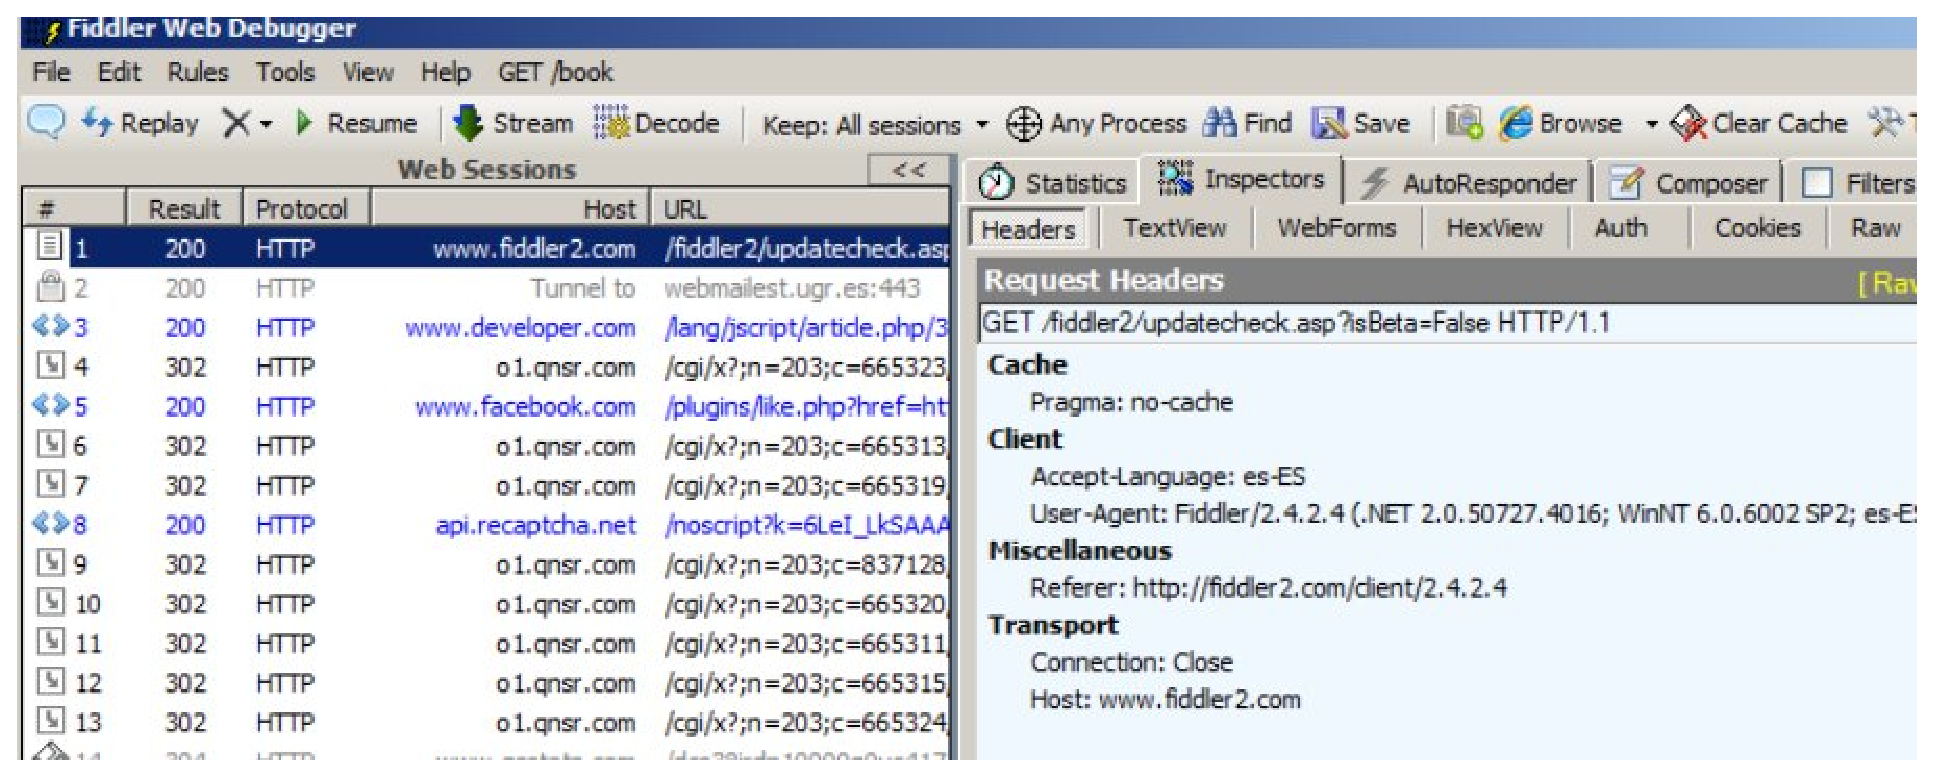
\includegraphics[scale=0.4]{imagenes/cuestion7-1.eps}
\caption{Vemos que no aparece informacion sobre las cabeceras.}
\end{center}
\end{figure}

Configuramos el IIS de forma que esé habilitado para la compresión de contenido estático de la siguiente manera:
\begin{figure}[H]
\begin{center}
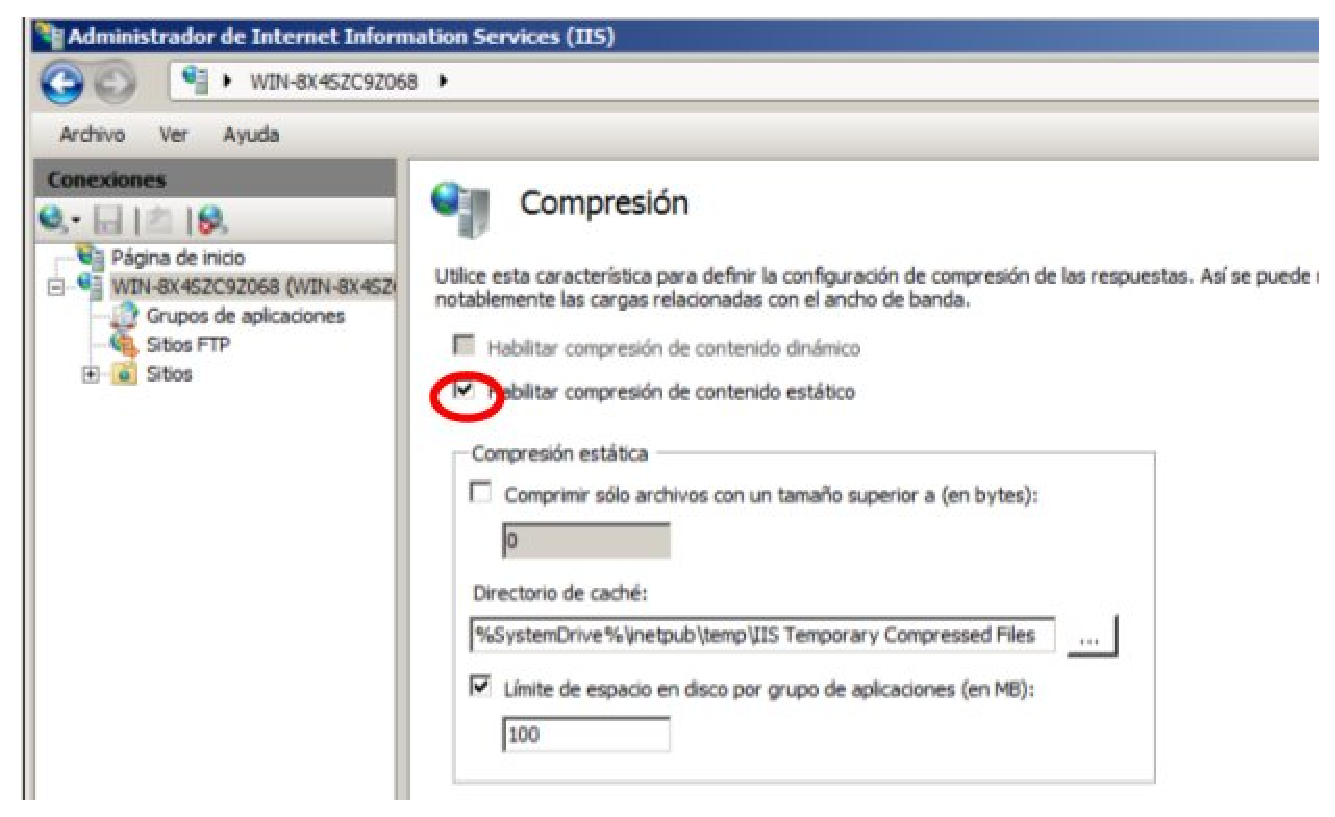
\includegraphics[scale=0.5]{imagenes/cuestion7-2.eps}
\caption{Habilitando compresión estática.}
\end{center}
\end{figure}

Y podemos comprobar que esta comprimo el contenido las páginas web, por ejemplo Facebook:
\begin{figure}[H]
\begin{center}
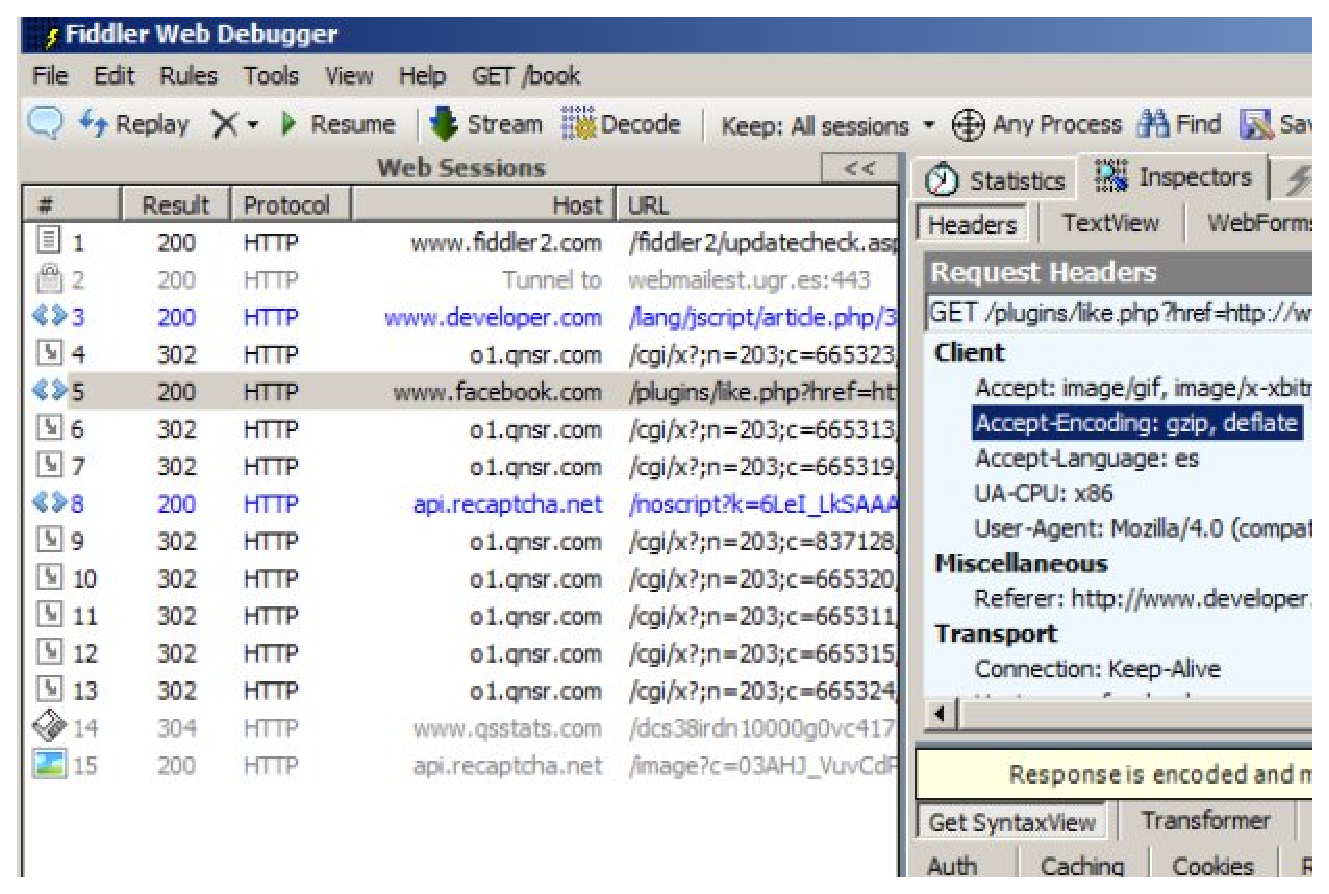
\includegraphics[scale=0.5]{imagenes/cuestion7-3.eps}
\caption{Comprobando compresión estática.}
\end{center}
\end{figure} 

\section{ Usted parte de un SO con ciertos parámetros definidos en la instalación (Práctica 1), ya sabe instalar servicios (Práctica 2) y cómo monitorizarlos (Práctica 3) cuando los somete a cargas (Práctica 4). Al igual que ha visto cómo se puede mejorar un servidor web (Práctica 5 Sección 3.1), elija un servicio (el que usted quiera) y modifique un parámetro para mejorar su comportamiento. (9.b) Monitorice el servicio antes y después de la modificación del parámetro aplicando cargas al sistema (antes y después) mostrando los resultados de la monitorización.}
\footnote{http://www2.tiendalinux.com/docs/manuales/redhat/rhl-rg-es-7.1/s1-configuration-config.html}

Como ya se han comentado en la cuestión 6 es posible cambiar gran cantidad de parámetros de un servidor Apache.

Entre estos, es de destacar, "MaxKeepAliveRequests" que establce el número máximo de peticiones permitidas por cada conexión. Es recomendable un valor alto según el grupo apache. El "Timeout" que define, en segundos, el tiempo que el servidor esperará  para recibir o enviar peticiones durante la comunicación. Y "MaxClients" que establece el limite de procesos del servidor \footnote{http://www2.tiendalinux.com/docs/manuales/redhat/rhl-rg-es-7.1/s1-configuration-config.html}.

Cambiaré los dos primeros para comprobar los resultados con ApacheBenchmark. Esto se realizará sobre mi servidor apache, creado en Ubuntu.
La página es un archivo html con algo de javascript, que he subido ha mi servidor.

El comando de ApacheBenchmark que he usado es el siguiente:

\textit{ab -n 1000 -c 100 http://localhost/pagina.html/}

En la primera ejecución los parámetros son :

Timeout 300
MaxKeepAliveRequests 100

Y el resultado mostrado  es el siguiente:

\begin{figure}[H]
\begin{center}
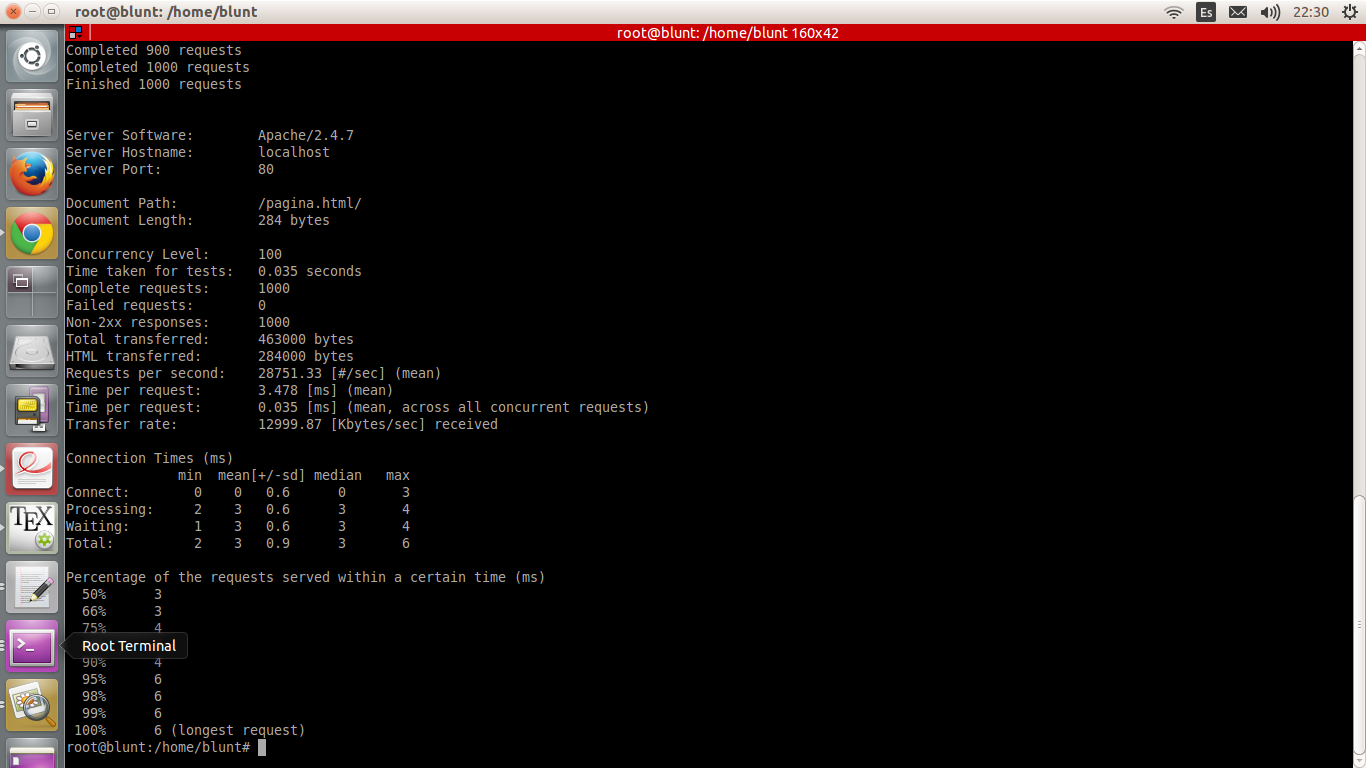
\includegraphics[scale=0.3]{imagenes/cuestion8-1.eps}
\caption{Resultados del sistema con "ab" antes.}
\end{center}
\end{figure}

En la segunda configuracion dejamos los siguientes valores:

Timeout 400
MaxKeepAliveRequest 50

Y el resultado es el siguiente:
\begin{figure}[H]
\begin{center}
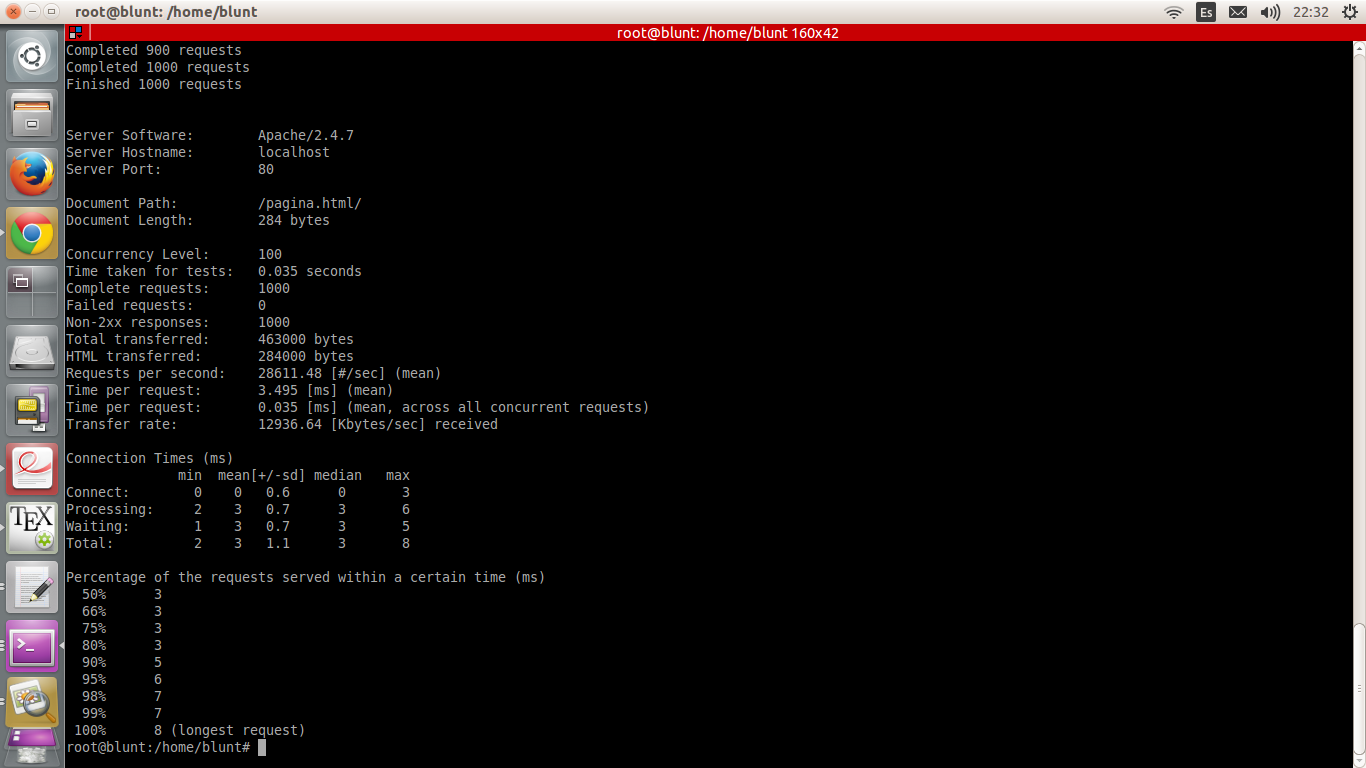
\includegraphics[scale=0.3]{imagenes/cuestion8-2.eps}
\caption{Resultados de "ab" con la primera configuración.}
\end{center}
\end{figure}

Para la última configuración los valores son :
Timeout 200
MaxKeepAliveRequest 150

Y los resultados :

\begin{figure}[H]
\begin{center}
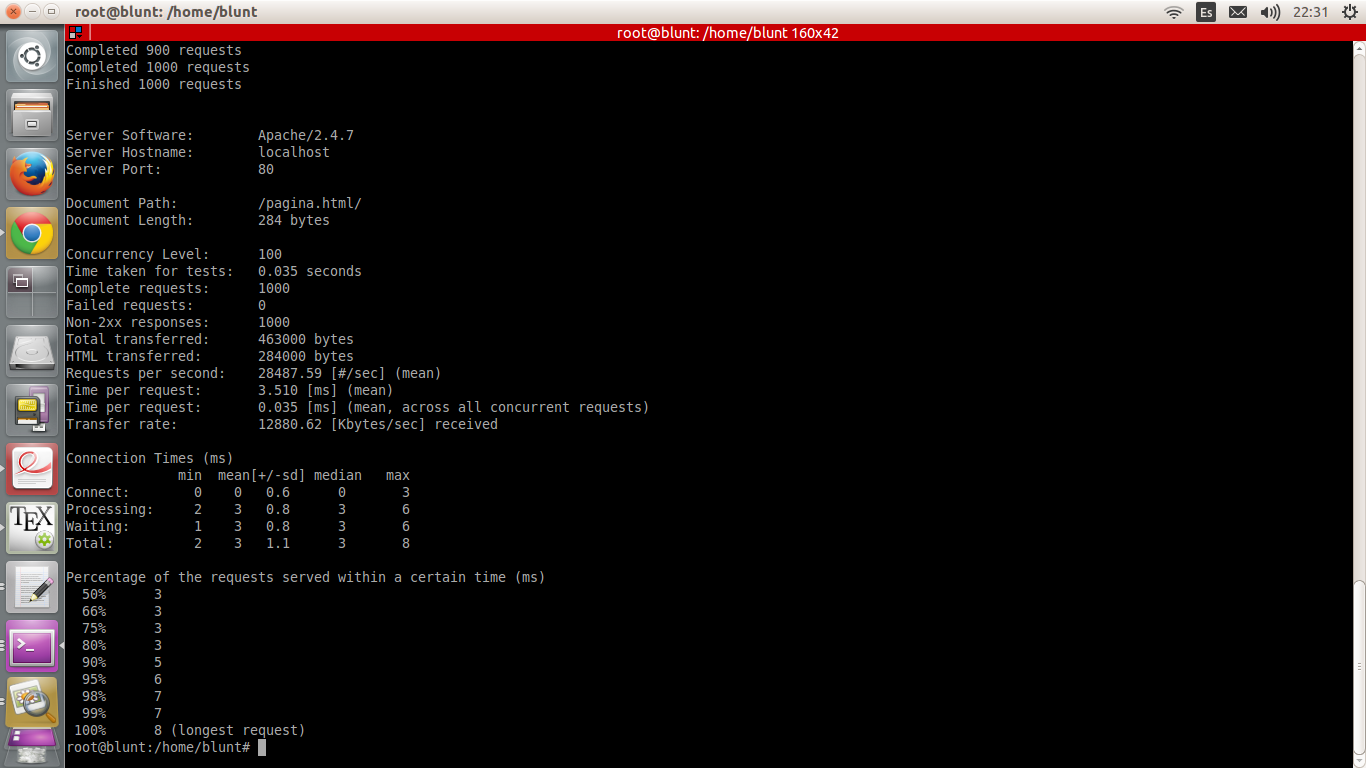
\includegraphics[scale=0.3]{imagenes/cuestion8-3.eps}
\caption{Resultados de "ab" para la segunda configuración.}
\end{center}
\end{figure}


Vemos como la configuración inicial que es la mas equilibrada recibe mejores resultados de tiempo, aunque estos no son muy significativos pues la página no es gran cosa.



\end{document}